\documentclass[10pt]{article} 
\usepackage{ctex}
\usepackage{graphicx}
\usepackage{amsmath}
\usepackage{epstopdf}
\usepackage{tabularx}
\usepackage{geometry}
\usepackage{float}
\usepackage{listings}
\usepackage{xcolor}
\usepackage{fontspec}
\usepackage{color}
\usepackage{caption}
\usepackage[dvipsnames]{xcolor}
\lstset{
	language = matlab,
	backgroundcolor = \color{yellow!10}, % 背景色:淡黄
	basicstyle = \small\ttfamily, % 基本样式 + 小号字体
	rulesepcolor= \color{gray}, % 代码块边框颜色
	breaklines = true, % 代码过长则换行
	numbers = left, % 行号在左侧显示
	numberstyle = \small, % 行号字体
	keywordstyle = \color{blue}, % 关键字颜色
	commentstyle =\color{green!60}, % 注释颜色
	stringstyle = \color{red!100}, % 字符串颜色
	frame = shadowbox, % 用(带影子效果)方框框住代码块
	showspaces = false, % 不显示空格
	columns = fixed, % 字间距固定
	%escapeinside={} % 特殊自定分隔符:
	morekeywords = {as}, % 自加新的关键字(必须前后都是空格)
	deletendkeywords = {compile} % 删除内定关键字;删除错误标记的关键用deletekeywords删!
}
\geometry{right=1cm,left=1cm,top=1cm,bottom=1.5cm}
\makeatletter
\newcommand*\@lbracket{[}
\newcommand*\@rbracket{]}
\newcommand*\@colon{:}
\newcommand*\colorIndex{%
    \edef\@temp{\the\lst@token}%
    \ifx\@temp\@lbracket \color{black}%
    \else\ifx\@temp\@rbracket \color{black}%
    \else\ifx\@temp\@colon \color{black}%
    \else \color{vorange}%
    \fi\fi\fi
}
\makeatother
\usepackage{trace}
\title{语音合成大作业}
\author{王炜致\ 2022010542}
\date{}
\begin{document}
\maketitle
\section{语音预测模型}
\subsection*{(1)}
\textbf{\color{gray}
给定$$e(n) = s(n) - a_1s(n - 1) - a_2s(n - 2)$$
假设 e(n) 是输入信号, s(n) 是输出信号, 上述滤波器的传递函数是什么? 如果 $a_1 = 1.3789
$,$a_2 = -0.9506$,上述合成模型的共振峰频率是多少?用zplane , freqz , impz分别绘出零
极点图,频率响应和单位样值响应。用 filter 绘出单位样值响应,比较和 impz 的是否相同。}

\textcircled{1}上述滤波器的传递函数为$$H(z)=\frac{1}{1-\frac{a_1}{z}-\frac{a_2}{z^2}} 
=\frac{z^2}{z^2-a_1z-a_2}$$

\textcircled{2}共振峰频率$$f=\frac{\omega}{2\pi}$$
而模拟频率$\omega$和数字频率$\Omega$有关系$$\Omega=\omega T$$
故$$f=\frac{\Omega}{2\pi T}\approx1kHz$$

\textcircled{3}用zplane,freqz分别绘出零极点图、频率响应
如下:
\begin{figure}[htbp]
	\centering
	\begin{minipage}{0.49\linewidth}
		\centering
		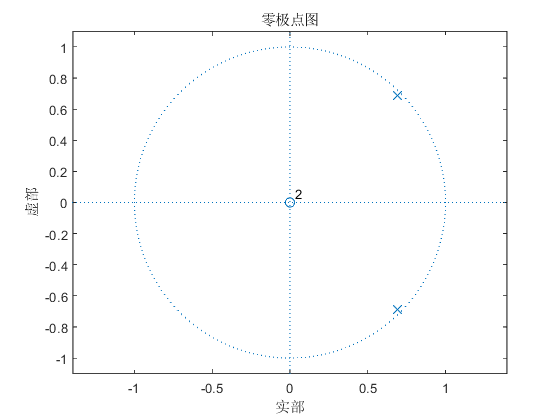
\includegraphics[width=0.9\linewidth]{drawing1-1.png}
		\caption{零极点图}
	\end{minipage}
	\begin{minipage}{0.49\linewidth}
		\centering
		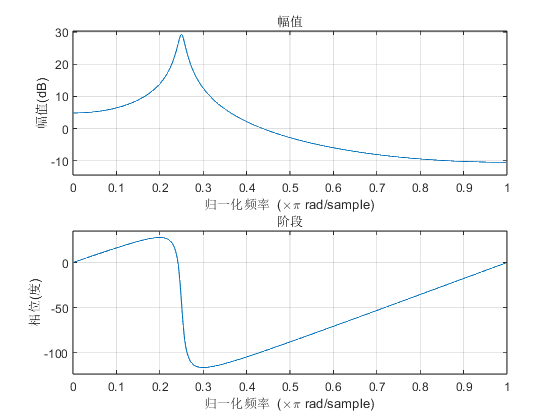
\includegraphics[width=0.9\linewidth]{drawing1-2.png}
		\caption{频率响应}
	\end{minipage}
	%\qquad
	%让图片换行,
\end{figure}

用impz,filter分别绘出单位样值响应如下,两者相同:
\begin{figure}[h]
	\centering
	\begin{minipage}{0.49\linewidth}
		\centering
		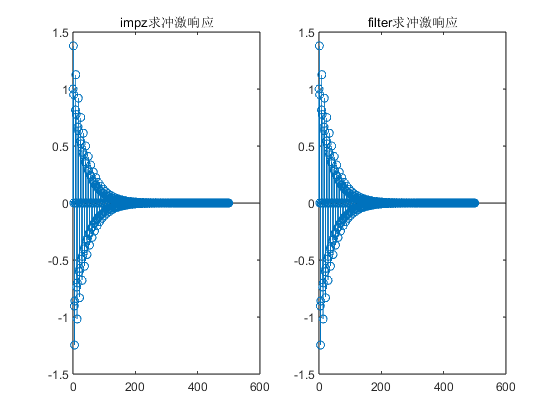
\includegraphics[width=0.9\linewidth]{drawing1-3.png}
		\caption{冲激响应}
	\end{minipage}
\end{figure}
\newpage
\subsection*{(3)((2)略)}
\textbf{\color{gray}运行程序到 27 帧时停住, 用(1) 中的方法观察零极点图。}

如下所示,用zplane函数绘制E,A决定的零极点图即可。注意A是预测系数,应用以表示z变换表达式的分母部分。
\begin{lstlisting}[language=matlab]
% (3) 在此位置写程序,观察预测系统的零极点图
    zplane(E,A);
    \end{lstlisting}

\begin{figure}[h]
	\centering
	\begin{minipage}{0.49\linewidth}
		\centering
		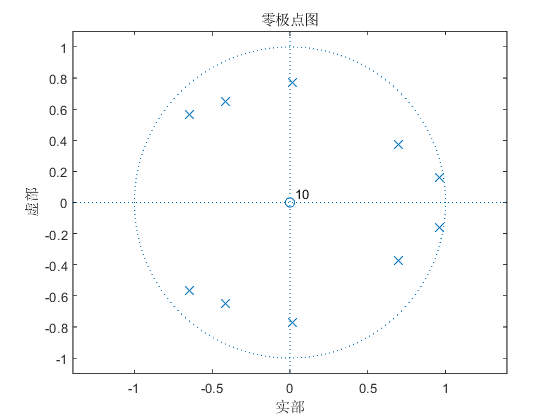
\includegraphics[width=0.9\linewidth]{coding1.png}
		\caption{27帧对应零极点图}
	\end{minipage}
\end{figure}

\subsection*{(4)}
\textbf{\color{gray}在循环中添加程序: 对每帧语音信号 s(n) 和预测模型系数 $\{a_i\} $, 用 filter 计算
激励信号 e(n) 。}

由于分帧处理,需要保存滤波器的最终条件zf,且需要考虑滤波器的初始状态zi,在代码中表现为更新zi\_pre
的值。注意求激励即预测残差需要将滤波器输入输出对换,A应作分子,1应作分母。
\begin{lstlisting}[language=matlab]
% (4) 在此位置写程序,用filter函数s_f计算激励,注意保持滤波器状态
    [exc_ftr,zi_pre] = filter(A,1,s_f,zi_pre);
    exc((n-1)*FL+1:n*FL) = exc_ftr;
% exc((n-1)*FL+1:n*FL) = ... 将你计算得到的激励写在这里
\end{lstlisting}
\subsection*{(5)}
\textbf{\color{gray}完善 speechproc.m 程序, 在循环中添加程序: 用你计算得到的激励信号 e(n) 和预
测模型系数 $\{a_i\} $ , 用 filter 计算重建语音 $\hat{s}(n)$ 。}

类似地有(注意输入输出):
\begin{lstlisting}[language=matlab]
% (5) 在此位置写程序,用filter函数和exc重建语音,注意保持滤波器状态
    [rec_ftr,zi_rec] = filter(1,A,exc_ftr,zi_rec);
    s_rec((n-1)*FL+1:n*FL) = rec_ftr;
% s_rec((n-1)*FL+1:n*FL) = ... 将你计算得到的重建语音写在这里
\end{lstlisting}

\subsection*{(6)}
\textbf{\color{gray}在循环结束后添加程序: 用 sound 试听(6) 中的 e(n) 信号, 比较和 s(n) 以及 $\hat{s}(n)$
信号有何区别。 对比画出三个信号, 选择一小段, 看看有何区别。}

信号所载信息均为“电灯比油灯进步多了”。
e(n)信号噪声较大;s(n)信号和$\hat{s}(n)$信号听起来几无区别,且两者噪声相对e(n)较小。因为
e(n)是语音信号s(n)和$\sum_{k=1}^{N}a_ks(n-k)$的差(残差),自然与s(n)相差较大;作为激励信号可以
较好重建语音。
\begin{figure}[h]
	\centering
	\begin{minipage}{0.49\linewidth}
		\centering
		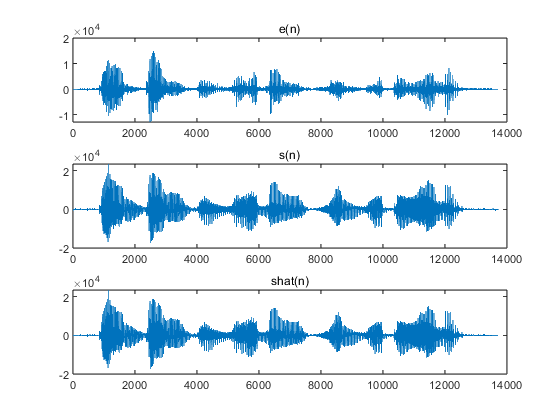
\includegraphics[width=0.9\linewidth]{compare.png}
		\caption{语音信号比较}
	\end{minipage}
\end{figure}

选取[2000,4000]局部区间比较,
\begin{figure}[h]
	\centering
	\begin{minipage}{0.49\linewidth}
		\centering
		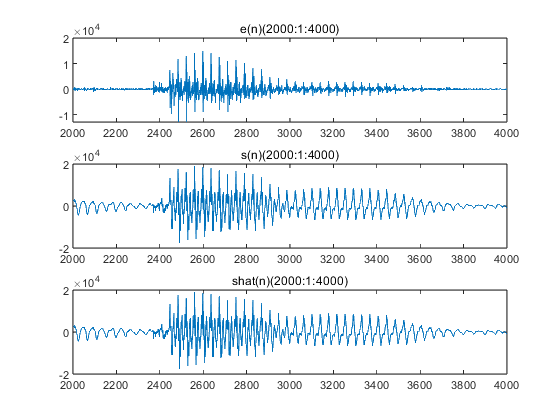
\includegraphics[width=0.9\linewidth]{commpare.png}
		\caption{语音信号比较(局部)}
	\end{minipage}
\end{figure}
进一步验证了前述判断:
\section{语音合成模型}
\subsection*{(7)}
\textbf{\color{gray}生成一个 8kHz 抽样的持续 1 秒钟的数字信号, 该信号是一个频率为 200Hz 的单
位样值“串”, 即$$x(n)=\sum_{i=0}^{NS-1}\delta(n-iN)$$考虑该信号的 N 和 NS 分别为何值? 
用 sound 试听这个声音信号。 再生成一个 300Hz 的单位样值“串”并试听, 有何区别? }

\textcircled{1}抽样频率的定义为单位时间内从连续信号中提取并组成离散信号的抽样个数。
故1s内的抽样点有8000个;该信号频率为200Hz,故$NS=200$,$N=\frac{8000}{200}=40$。
定义抽样频率
\begin{lstlisting}[language=matlab]
fsp=8000;
\end{lstlisting}
则用sound试听声音信号的代码为(注意到sound默认声音时长为1s)
\begin{lstlisting}[language=matlab]
seq1=zeros(fsp,1);
f1=200;
pulse1=floor(fsp/f1);
for n=1:f1 %matlab start from 1
    seq1(pulse1*n)=1;
end
sound(seq1);
\end{lstlisting}

\textcircled{2}同上,信号频率为300Hz时,$NS=300$,$N=\frac{8000}{300}=26$,试听代码为
\begin{lstlisting}[language=matlab]
seq2=zeros(fsp,1);
f2=300;
pulse2=floor(fsp/f2);
for n=1:f2 %matlab start from 1
    seq2(pulse2*n)=1;
end
sound(seq2);
	\end{lstlisting}

注意到,300Hz信号的音调显著地比200Hz音调要高。

\subsection*{(8)}
\textbf{\color{gray}真实语音信号的基音周期总是随着时间变化的。我们首先将信号分成若干个 10
毫秒长的段, 假设每个段内基音周期固定不变,但段和段之间则不同,具体为
$$PT = 80 + 5mod(m,50)$$
其中PT表示基音周期, m表示段序号。生成1秒钟的上述信号并试听。}

由于段长为10ms,总长为1s,易知信号的段数为100,则信号生成并试听的代码为
\begin{lstlisting}[language=matlab]
fsp=8000; N=100;
seq=zeros(fsp,1); n=1;
while n<=fsp
    seq(n)=1;
    m=ceil(n/(fsp/N));
    PT=80+5*mod(m,50);
    n=n+PT;
end
sound(seq);
\end{lstlisting}
相邻两个脉冲间的PT值由更靠前的那个脉冲(所在的段号)决定。

\subsection*{(9)}
\textbf{\color{gray}用 filter 将(8) 中的激励信号 e(n) 输入到(1) 的系统中计算输出 s(n) , 试听和
e(n) 有何区别。}

试听比较,发现有显著变化,通过图像进一步观察其变化情况。将e(n)视为一系列冲激信号
的叠加,则s(n)则对应为各冲激信号响应的叠加。各个冲激信号及其响应情况与[图3:冲激响应
]所示大体上是吻合的。
\begin{figure}[h]
	\centering
	\begin{minipage}{0.49\linewidth}
		\centering
		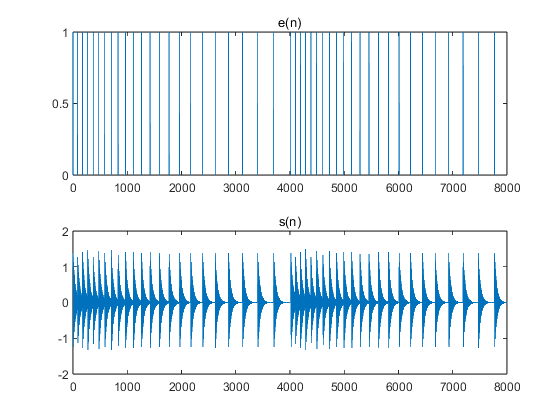
\includegraphics[width=0.7\linewidth]{drawing2-9.png}
		\caption{输入e(n)与输出s(n)信号比较}
	\end{minipage}
\end{figure}
\subsection*{(10)}
\textbf{\color{gray}重改 speechproc.m 程序。 利用每一帧已经计算得到的基音周期和(8) 的方法,
生成合成激励信号 Gx(n)( G 是增益), 用 filter 函数将 Gx(n) 送入合成滤波器得到合成语
音 s~(n) 。 试听和原始语音有何差别。}

帧长FL=80。模仿(8)中代码,在循环开始前预置k=2FL+1(即从第3帧开始):
\begin{lstlisting}[language=matlab]
k = 2*FL + 1;
\end{lstlisting}
k作为下标,为合成激励信号exc\_syn在适当位置添加加权脉冲,具体操作如下:
\begin{lstlisting}[language=matlab]
while k <= FL*n
    exc_syn(k) = G;
    k = k + PT;
end
\end{lstlisting}
k按照已经计算好的PT跳跃,在当前帧添加加权脉冲,当超过当前帧范围时结束,
完成当前帧激励信号的合成。

将当前帧激励信号输入滤波器(注意保存状态),即得合成语音$\tilde{s}(n)$:
\begin{lstlisting}[language=matlab]
[s_syn((n-1)*FL+1:n*FL),zi_syn] = filter(1,A,exc_syn((n-1)*FL+1:n*FL),zi_syn);
\end{lstlisting}
\begin{figure}[h]
	\centering
	\begin{minipage}{0.49\linewidth}
		\centering
		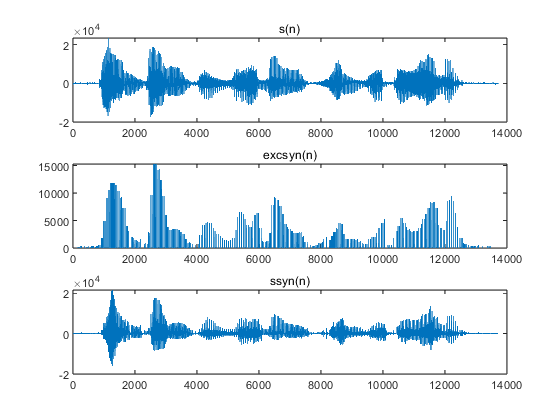
\includegraphics[width=0.7\linewidth]{drawing2-10.png}
		\caption{合成信号比较}
	\end{minipage}
\end{figure}
听觉上,s(n)与$\tilde{s}(n)$无明显不同,观察图像发现s(n)局部幅度更大些,
其余差异亦不显著。

\section{变速不变调}
\subsection*{(11)}
\textbf{\color{gray}仿照(10) 重改 speechproc.m 程序, 只不过将(10) 中合成激励的长度增加一倍,
即原来 10 毫秒的一帧变成了 20 毫秒一帧, 再用同样的方法合成出语音来。}

将n统一改为2n即可:
\begin{lstlisting}[language=matlab]
% (11) 不改变基音周期和预测系数,将合成激励的长度增加一倍,再作为filter
% 的输入得到新的合成语音,听一听是不是速度变慢了,但音调没有变。
while k_v <= FL*n*2
    exc_syn_v(k_v) = G;
    k_v = k_v + PT;
end

[s_syn_v(2*(n-1)*FL+1:2*n*FL),zi_syn_v] = filter(1,A,exc_syn_v(2*(n-1)*FL+1:2*n*FL),zi_syn_v);
\end{lstlisting}
\begin{figure}[h]
	\centering
	\begin{minipage}{0.49\linewidth}
		\centering
		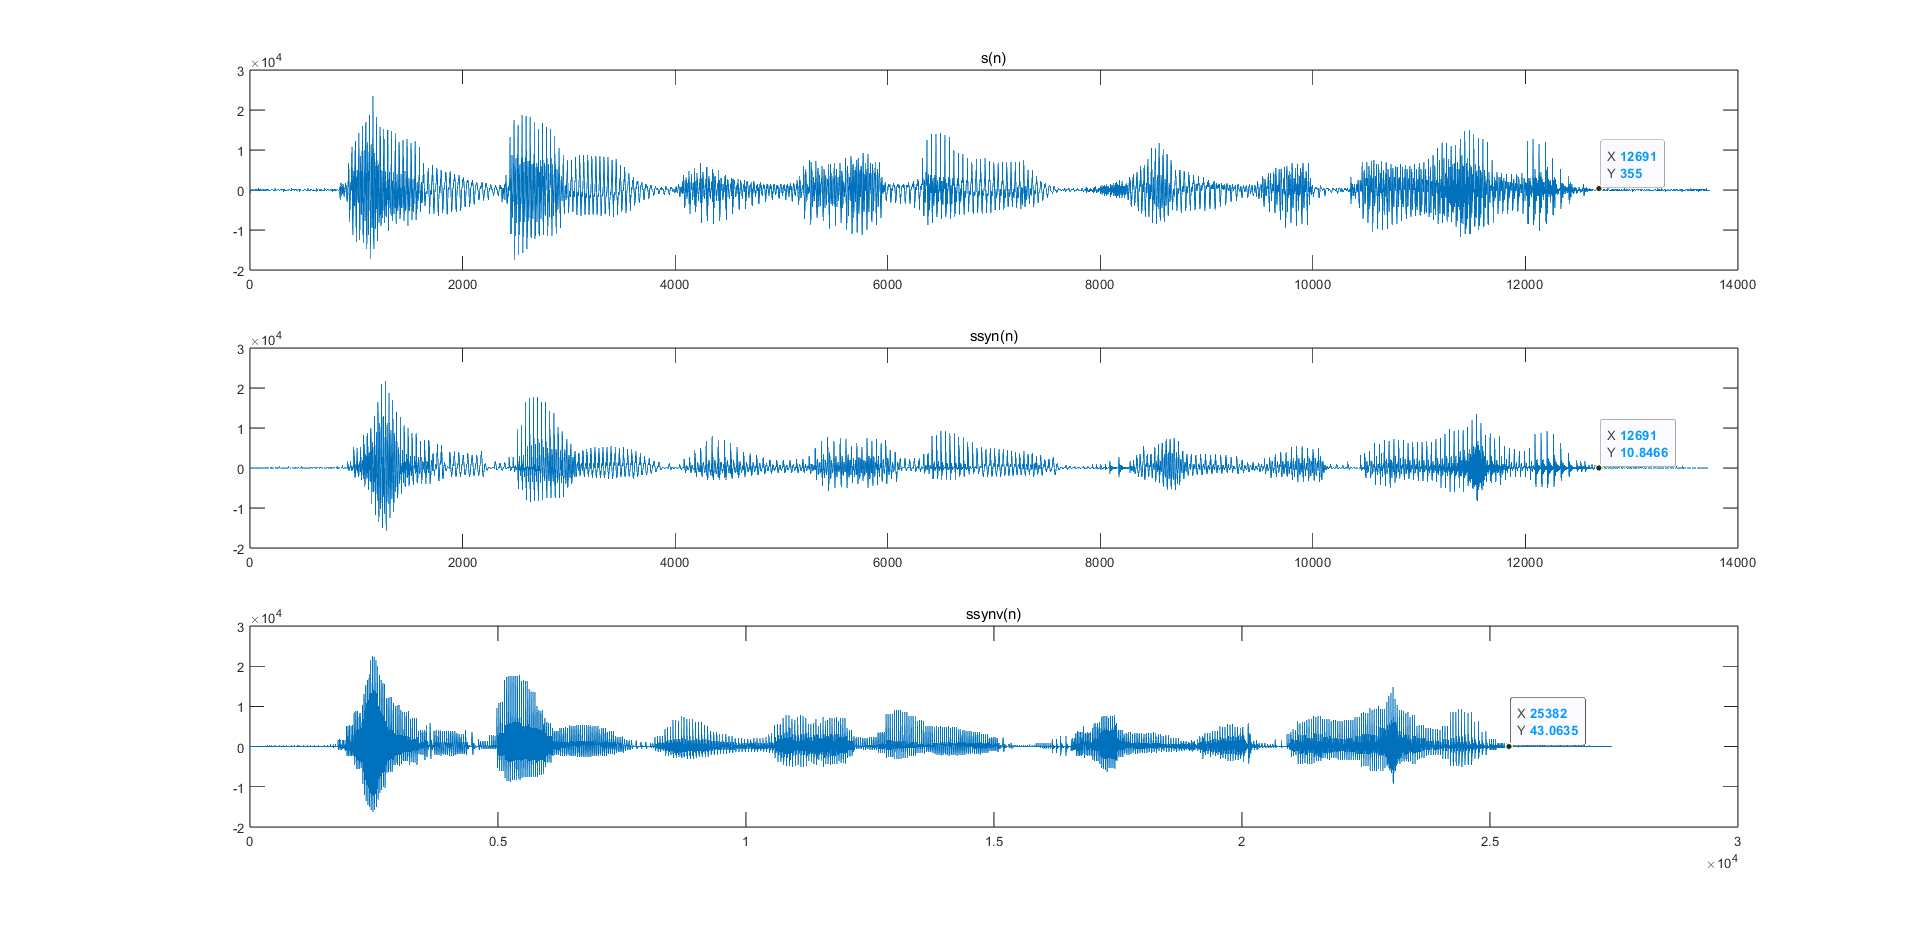
\includegraphics[width=1\linewidth]{drawing2-11.png}
		\caption{合成信号比较}
	\end{minipage}
\end{figure}
听取语音,记录两个语音(s,s\_v)播放的大致时间,以及观察图像横坐标,可知信号长度确实增加了一倍;
此外音调并无明显变化,说明实现了变速不变调。

\subsection*{(12)}
\textbf{\color{gray}重新考察(1) 中的系统, 
将其共振峰频率提高 150Hz 后的 $a_1$ 和 $a_2$ 分别是多少?}

\end{document}